\documentclass[french]{article}

\usepackage[french]{babel}

\usepackage[utf8]{inputenc}
\usepackage[T1]{fontenc}
\usepackage[hidelinks]{hyperref}
\usepackage{graphicx}
\usepackage{amsmath}
\usepackage[left=1.3in,right=1.3in]{geometry}
\usepackage{microtype}
\usepackage{upquote}
\usepackage{listings}
\usepackage{url}
\usepackage[backend=biber]{biblatex}

\usepackage{pdfpages}

\usepackage{titling}
\newcommand{\subtitle}[1]{%
  \posttitle{%
    \par\end{center}
    \begin{center}\large#1\end{center}
    \vskip0.5em}%
}

\addbibresource{references.bib}

\title{Martine résout le problème du voyageur de commerce}
\subtitle{Avec un algorithme A*}
\author{Maxence \textsc{Aïci} \and Rémi \textsc{Nicole}}

\begin{document}

\maketitle

\tableofcontents

\part{Modélisation}

\paragraph{} Le problème du voyageur de commerce est probablement le problème
NP-complet le plus connu en algorithmique, mais dans le doute, voici la
définition de Wikipedia~\cite{wiki:tsp}:

\begin{quote}
	``Given a list of cities and the distances between each
	pair of cities, what is the shortest possible route that visits each city
	exactly once and returns to the origin city?''
\end{quote}

\paragraph{} Quant aux algorithmes de type A*, il s'agit tout simplement d'une
amélioration de l'algorithme de Dijkstra qui choisit sans aucun scrupule les
sommets qui sont le plus susceptible de nous mener à la solution optimale. On
calcule cette ``susceptibilité'' grâce à une heuristique qui calculera de
manière arbitraire une estimation du score restant pour aller à l'arrivée.

De manière mathématique, parce qu'en algorithmie, on aime bien écrire des
équations compliquées, et en plus en \LaTeX, ça nous donne un rendu magnifique:

\[f(n) = g(n) + h(n)\]

Avec:
\begin{itemize}
	\item $n$ l'étape par laquelle l'algorithme suggère de passer
	\item $f(n)$ l'estimation du coût total en passant par l'étape $n$
	\item $g(n)$ le coût d'aller du début jusqu'à l'étape $n$
	\item $h(n)$ l'estimation du coût pour aller de l'étape $n$ à l'arrivée
\end{itemize}

\section{Graphe de résolution de problème}

\paragraph{} Tout d'abords, il nous faut un arbre de résolution de problème
pour pouvoir faire de l'A*. Nous le définissons donc ainsi:

Si la carte des villes ressemble à ceci:
\begin{center}
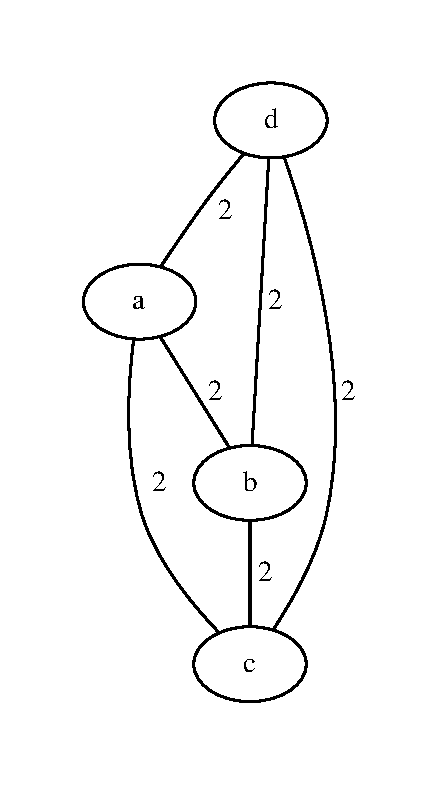
\includegraphics[scale=0.5]{graphs/modeling-the-problem_example1-map.pdf}
\end{center}

Alors on aura notre graphe de résolution de problème, ou PSG pour l'acronyme
anglais (aucune affiliation avec aucun groupe sportif), qui sera:
\begin{center}
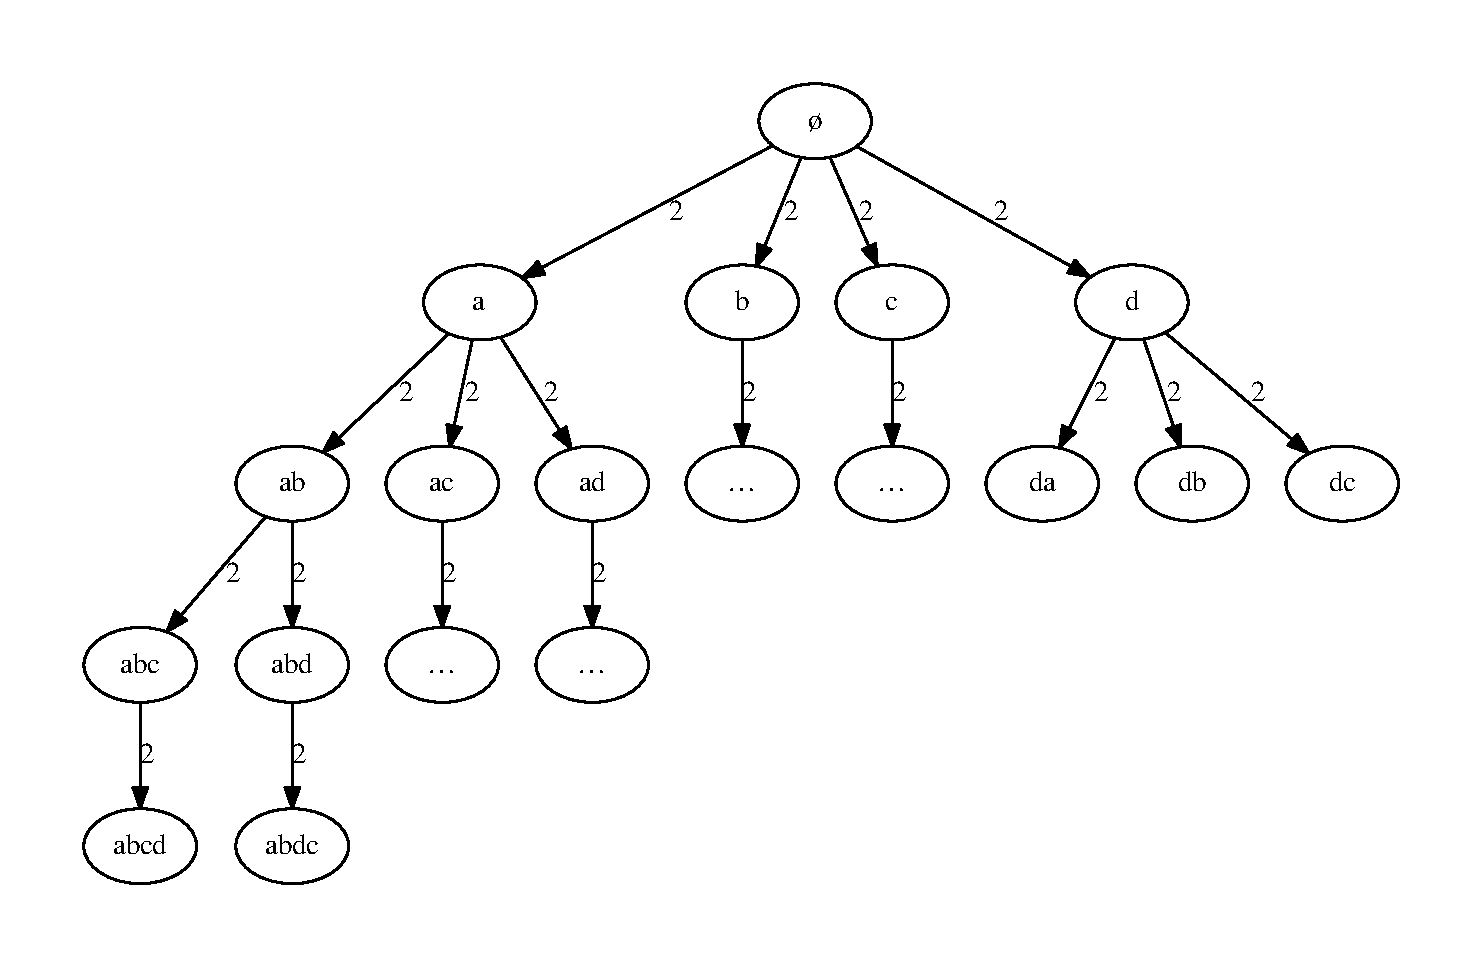
\includegraphics[scale=0.5]{graphs/modeling-the-problem_example1-psg.pdf}
\end{center}

Et, par exemple, après avoir pris le chemin A $\rightarrow$ B $\rightarrow$ C,
on aura:
\begin{center}
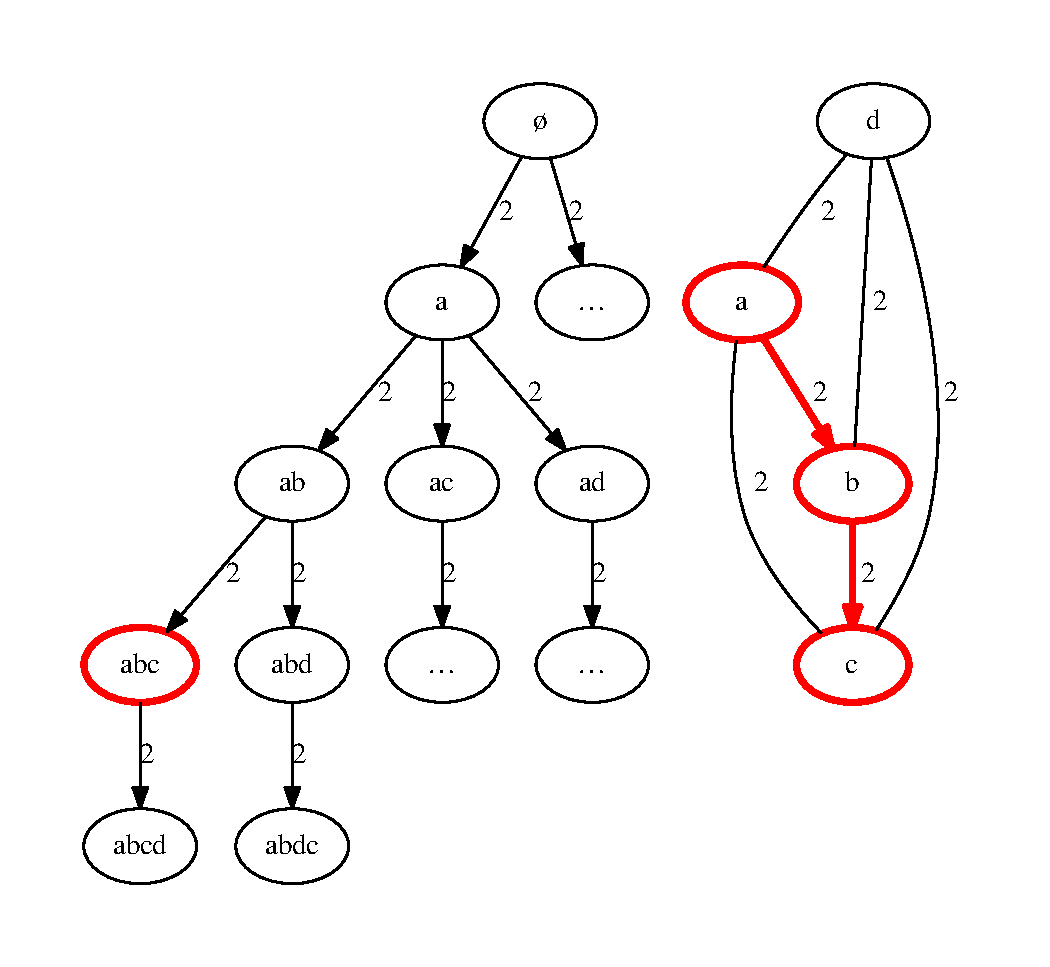
\includegraphics[scale=0.5]{graphs/modeling-the-problem_example2.pdf}
\end{center}

\section{Heuristiques}

\paragraph{} Pour ne pas être aussi inefficace que Dijkstra et pouvoir enfin
s'appeler A*, parce qu'avoir un nom prononçable c'est aussi important, il nous
faut des heuristiques. Il est aussi important d'avoir des heuristiques qui
estiment suffisamment bien le poids du chemin restant, mais tout en restant
facile à calculer parce que l'on risque d'en avoir souvent besoin au cours de
l'algorithme.

\subsection{Nulle}

\paragraph{} Comme son nom l'indique, l'heuristique nulle n'est pas terrible.
Il s'agit tout simplement de l'heuristique qui n'estime pas. En dehors d'être
le Saint Graal des heuristiques pour programmeurs fainéants, elle nous servira
aussi à tester notre algorithme, qui se ramènera donc à Dijkstra, nom qui,
cette fois ci, m'a fait reprendre à trois fois avant de pouvoir le taper
correctement.

\subsection{Arête de poids minimum}

\paragraph{} Une autre heuristique simple, mais pas autant que précédemment,
est de prendre l'arête de poids minimum dans la carte privée des villes
parcourues, et de le multiplier par le nombre de villes restant à parcourir. Ce
n'est pas vraiment une bonne approximation, mais au moins on est sûr que le
chemin optimal aura comme borne inférieure le résultat de cette heuristique.

\subsection{Dijkstra}

\paragraph{} Curieuse coïncidence, on peut utiliser Dijsktra dans une
heuristique A*. Cette heuristique consiste à prendre le plus cours chemin de la
ville actuelle jusqu'à la ville de départ. Avec un peu de chance cette
approximation sera exacte, même si la complexité laisse à désirer.

\subsection{Arbre de poids minimum}

\paragraph{} Une utilisation intéressante de l'arbre de poids minimum, ou MST
pour l'acronyme anglais que l'on ne commentera pas, est de l'intégrer dans une
heuristique du voyageur de commerce. De plus, si l'on fait les bons choix
d'implémentation, il a une complexité de:

\[O(|\text{arêtes}| \times \log\left(|\text{sommets}|\right))\]

ce qui pourrait être un bon compromis entre la précision de l'approximation et
la complexité de l'heuristique.

Une fois que le MST de la carte, toujours privée des villes déjà parcourues,
est obtenu, il nous suffira de sommer le poids des arêtes et on aura notre
approximation!

\part{Implémentation des structures}

\paragraph{} Afin d'implémenter (ou d'implanter pour les gens bizarres)

\part{Implémentation de l'algorithme}

\part{Tests}

\part{Jouer à Hercule Poirot}

\printbibliography%

\end{document}
